\section{Empirical Methodology}
\label{sec:empirical}
To evaluate the HIGHLIGHTS and HIGHLIGHTS+DIV algorithms, we generated summaries for agents playing the Mrs. Pacman game.  
%To measure people's ability to assess the capabilities of different agents, we used an agent comparison task where participants were shown summaries of two agents and  were asked to choose which agent they want to play on their behalf
In addition to using the two versions of the HIGHLIGHTS algorithm to generate summaries, we also generated summaries with two baseline methods:
\begin{itemize}
\item \emph{First}: a summary is generated from the first $k$ trajectories Pacman encounters. This baseline corresponds to the user watching the agent act (e.g., watching a video of an autonomous vehicles driving) until she runs out of time.
\item \emph{Random}: a summary is generated by sampling $k$ trajectories uniformly from the agent's execution trace. Since we generate the summaries online, we used reservoir sampling~\cite{vitter1985random} which extracts random samples from an online stream. On average, this baseline will sample states based on the frequency of encountering them (a state that is more frequently encountered is more likely to be selected to the summary). 
\end{itemize}
In the experiments, we used a budget of $k = 5$ and a trajectory length $l=40$, meaning that all summaries included five trajectories, each showing 40 neighboring states. We used $statesAfter=10$, meaning that each trajectory included 10 states following the important state (the first 29 states were the states preceding the important state). All methods enforced a gap of 50 states before considering a state for inclusion in the summary (i.e., $intervalSize = 50$).

We note that the summaries shown to participants did not include the current score of the agent (i.e., we removed the bottom part shown in Figure~\ref{fig:pacman}) such that their evaluation will not be based just on observing scores, but rather on the behavior of the Pacman player that they observed. 

Participants completed two types of task, described in more detail in Section~\ref{sec:procedure}. In the first task, participants were shown summaries of two different agents, and were asked to choose which agent they want to play on their behalf. This task provides an objective way of assessing whether the summaries helped participants assess the performance of different agents. In the second task, participants were shown two summaries of \emph{the same} agent, and were asked which summary they found more helpful for assessing the agent's capabilities. This task provided a subjective measure assessing the perceived usefulness of the summaries. For these tasks, we generated three different agents by varying their training period. The lowest performing agent was trained for 200 episodes, the medium agent for 400 episodes, and the highest performing agent was trained fro 2000 episodes. Henceforth we refer to these agents as the \emph{200E}, \emph{400E} and \emph{2000E} agent, respectively. Generating agents of varying performance enabled us to have a ground truth for the agent selection task. The summaries were generated after the agents were fully trained, such that they reflect the final policies of the agents.  

We conducted two experiments. Experiment 1 compared summaries generated by the basic HIGHLIGHTS algorithm with summaries generated by the two baseline methods. Experiment 2 compared summaries generated by the HIGHLIGHTS+DIV algorithm with summaries generated by the basic HIGHLIGHTS algorithm and by the \emph{Random} baseline. In this section, we describe the Mrs. Pacman domain and the experimental procedure which was used in both Experiment 1 and Experiment 2. 

\subsection{The Mrs. Pacman Domain}
We generated summaries for agents playing the Mrs. Pacman game~\cite{rohlfshagen2011ms}. Figure~\ref{fig:pacman} shows the game maze used in our experiments. This game configuration includes two types of food pellets: regular pellets (small dots) are worth 10 points each and power pellets (larger dots) are worth 50 points each. After eating a power pellet, ghosts become edible for a limited time period. Pac-Man receives 200 points for each ghost it eats. Ghosts chase Pac-Man with $80\%$ probability and otherwise move randomly. In each state, Pac-Man has at most four moves (right, left, up or down). 

\begin{figure}
	\centering
	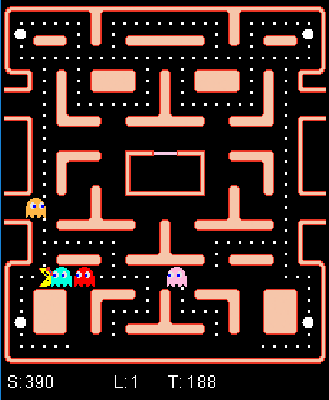
\includegraphics[width=0.4\columnwidth]{figs/pacman1.pdf}\\
	\caption{The Mrs. Pac-Man Game.}
	\label{fig:pacman}
	\vspace{-0.4cm}
\end{figure}

Due to the large size of the state space, we used a high-level feature representation for state-action pairs. Specifically, we use the 7-feature representation from Torrey \& Taylor's~\shortcite{torrey2013teaching} implementation. Q-values are defined as a weighted function of the feature values $ f_{i}(s,a)$:
\begin{equation}
Q(s,a)=\omega_{0}+\sum_{i}{\omega_{i} \cdot f_{i}(s,a)}
\label{e:q}
\vspace{-0.3cm}
\end{equation}

To generate Pacman agents of varying capabilities, we ran the SARSA reinforcement learning algorithm, varying the length of the training period. We generated 3 different agents: (1) an agent trained for 200 episodes; (2) an agent trained for 400 episodes, and (3) an agent trained for 2000 episodes. We chose these thresholds as they empirically resulted in differing qualitative performance. For example, the agent trained for 2000 episodes learned that eating ghosts provides a large reward, while the other two did not. In Pacman, important states (as defined in Equation~\ref{eq:importance}) might correspond to situations where Pacman is very close to ghosts or  when Pacman has an opportunity to eat a power pill, or a ghost. 
%Note that because the summaries are based on the different agent's simulations, agents of varying performance will likely encounter different states (e.g., the agent trained for 200 episodes might never eat a ghost). Furthermore, because the importance judgment is based but also assign them with different 



% In the experiment, we used a budget of $k = 5$, meaning that all summaries included five trajectories. All methods enforced a gap of 40 states before considering a state for inclusion in the summary. This constraint aimed to ensure that trajectories do not substantially overlap (which will likely result in less diverse summaries). Example summaries generated by the different methods can be viewed at ***add url***. 

%\subsection{Participants}
%We recruited 40 participants through Amazon Mechanical Turk. Participants received \$1.5 base rate payment. They were able to earn an additional bonus of up to \$0.9 based on their performance (explained in Section~\ref{sec:procedure}).  ***add demographics***



\subsection{Procedure}
\label{sec:procedure}
Participants were first shown a tutorial explaining the rules of the Pacman game and scoring. They then had to pass a quiz ensuring they read and understood the rules. Once they passed the quiz they were asked to complete two different tasks described next. We used a within-subject study design, such that all participants were presented with all summary methods. 
%An anonymized version of the study (without the consent form) can be accessed here ***add url***. 

\textbf{Task 1: Agent Selection.}
In the first task, participants were shown pairs of video summaries of two different Pacman agents, and were asked to choose the agent they would like to play on their behalf. In each pair, the videos were for different agents   but generated by the same summarization method (e.g., a HIGHLIGHTS summary of the \emph{200E} agent and a HIGHLIGHTS summary of the \emph{400E}). Overall, there were 9 such pairs (3 agent levels X 3 summarization methods). The different agent comparisons varied in the difficulty of identifying the better agent: the \emph{200E} and \emph{400E} agents had the most similar performance, resulting in a \emph{high-difficulty} comparison; the \emph{200E} and \emph{2000E} agents differed most substantially in their performance, resulting in a \emph{low-difficulty} comparison; we refer to the comparison of  the \emph{400E} and \emph{2000E} agents as the \emph{medium-difficulty} comparison, as the differences in the agents' policies were more substantial than for the \emph{200E} and \emph{400E} agents, but less substantial than for the \emph{200E} and \emph{2000E} agents. 

Participants were given bonus of 10 cents for each correct agent selection, such that they had a monetary incentive to select the correct agent. In addition to stating which agent they choose, participants were also asked to explain their selection and to rate their confidence in the agent selection on a 7-point Likert scale (1 - not at all confident to 7 - very confident). The ordering of pairs to compare as well as which summary was shown on the left and which on the right were counter-balanced. 

\textbf{Task 2: Summary Preference.}
While the first task assessed participants' objective ability to identify the better agent, in the second task we elicited participants subjective summary preference. They were again shown pairs of videos summarizing a Pacman's agent behavior, but this time the two video summaries were of \emph{the same} agent (and participants were told it was the same agent). Participants were asked to rate which of the summaries they find more helpful for assessing the Pacman agent capabilities using a 7-point Likert scale (1 - video A is more helpful to 7 - video B is more helpful). They were also asked to provide a short explanation of their preference. 

To maintain a reasonable experiment length and because we were primarily interested in the usefulness of Highlights summaries, in this task participants only made 4 comparisons (2 agent levels, comparing for each highlights with random and highlights with first). The ordering of pairs to compare as well as which summary was shown on the left and which on the right were randomized. 

\subsection{Evaluation Metrics and Analyses}
For task 1, we evaluated participants' correctness rate when selecting Pacman agents with each summary method. We analyzed the data using a logistic regression, controlling for the comparison type (200E vs. 400E agents, 400E vs. 2000E agents or 200E vs. 2000E agents). Since we used a within-subject design, we ran a repeated measures logistic regression. We also compared participants' confidence in making these selections. Confidence ratings were analyzed using an ordinal logistic regression, again controlling for the comparison type. 

The fitted models (both logistic regression and for ordinal logistic regression) can be meaningfully interpreted by considering the \emph{odds ratio} ($OR$) values of the regression coefficients of the independent variables\footnote{Odds ratio values are computed by exponentiating the regression coefficients, which estimate log odds ratios.}, which we report in the Results section. Odds ratios can be interpreted as effect sizes. Values between 1.5 and 3 are interpreted as a small effect, between 3 and 5 as medium, and above 5 as large~\cite{borenstein2009converting,chen2010big}.

For task 2, we compared the helpfulness ratings given to the summaries. We normalized the preferences such that 7 always means ``highlights is more helpful'' and 1 means ``baseline is more helpful''. That is, a rating greater than 4 indicates a preference for HIGHLIGHTS. We analyzed these ratings using the non-parametric Wilcoxon rank sum test~\footnote{We used Wilcoxon rank sum as the scale was ordinal and the data was not normally distributed. However, we obtain similar results when using standard t-test.}.




